%%
%% This is file `tikzposter-template.tex',
%% generated with the docstrip utility.
%%
%% The original source files were:
%%
%% tikzposter.dtx  (with options: `tikzposter-template.tex')
%%
%% This is a generated file.
%%
%% Copyright (C) 2014 by Pascal Richter, Elena Botoeva, Richard Barnard, and Dirk Surmann
%%
%% This file may be distributed and/or modified under the
%% conditions of the LaTeX Project Public License, either
%% version 2.0 of this license or (at your option) any later
%% version. The latest version of this license is in:
%%
%% http://www.latex-project.org/lppl.txt
%%
%% and version 2.0 or later is part of all distributions of
%% LaTeX version 2013/12/01 or later.
%%


\documentclass{tikzposter} %Options for format can be included here

\usepackage{todonotes}

\usepackage[tikz]{bclogo}
\usepackage{lipsum}
\usepackage{amsmath}

\usepackage{booktabs}
\usepackage{longtable}
\usepackage[absolute]{textpos}
\usepackage[it]{subfigure}
\usepackage{graphicx}
\usepackage{cmbright}
%\usepackage[default]{cantarell}
%\usepackage{avant}
%\usepackage[math]{iwona}
\usepackage[math]{kurier}
\usepackage[T1]{fontenc}


%% add your packages here
\usepackage{hyperref}
% for random text
\usepackage{lipsum}
\usepackage[english]{babel}
\usepackage[pangram]{blindtext}

\colorlet{backgroundcolor}{blue!10}

 % Title, Author, Institute
\title{Jigsaw Unintended Bias in Toxicity Classification}
\author{Pengcheng jiang$^1$}
\institute{$^1$ JiLin University, China \\
}
%\titlegraphic{logos/tulip-logo.eps}

%Choose Layout
\usetheme{Wave}

%\definebackgroundstyle{samplebackgroundstyle}{
%\draw[inner sep=0pt, line width=0pt, color=red, fill=backgroundcolor!30!black]
%(bottomleft) rectangle (topright);
%}
%
%\colorlet{backgroundcolor}{blue!10}

\begin{document}


\colorlet{blocktitlebgcolor}{blue!23}

 % Title block with title, author, logo, etc.
\maketitle

\begin{columns}
 % FIRST column
\column{0.5}% Width set relative to text width

%%%%%%%%%% -------------------------------------------------------------------- %%%%%%%%%%
 %\block{Main Objectives}{
%  	      	\begin{enumerate}
%  	      	\item Formalise research problem by extending \emph{outlying aspects mining}
%  	      	\item Proposed \emph{GOAM} algorithm is to solve research problem
%  	      	\item Utilise pruning strategies to reduce time complexity
%  	      	\end{enumerate}
%%  	      \end{minipage}
%}
%%%%%%%%%% -------------------------------------------------------------------- %%%%%%%%%%


%%%%%%%%%% -------------------------------------------------------------------- %%%%%%%%%%
\block{Introduction}{

  \begin{center}
    {Jigsaw Unintended Bias in Toxicity Classification}
  \end{center}
    \begin{itemize}
      \item given: A tagged dataset containing comments.Target 0 for malicious comments and 1 for friendly comments.
      \item target: detect toxic comments and minimize unintended model bias.
      \item evaluation: acc
    \end{itemize}
    
  
}
%%%%%%%%%% -------------------------------------------------------------------- %%%%%%%%%%


%%%%%%%%%% -------------------------------------------------------------------- %%%%%%%%%%
\block{text preprocess}{
\begin{description}
  \item[count]:Count the total number of words contained in all texts, the maximum and minimum number of words contained in a text
  \item[missing data]:Check for missing data
  \item[full]:Change abbreviations to full:isn't > is not(via dictionnary)
  \item[numbers]:clean numbers
  \item[alphabetic]:Find all non alphabetic characters and clean special chars
  \item[misspelling]:Solve the problem of misspelling words
  \item[lower]:lower the text
\end{description}
}
%%%%%%%%%% -------------------------------------------------------------------- %%%%%%%%%%


%%%%%%%%%% -------------------------------------------------------------------- %%%%%%%%%%

%\note{Note with default behavior}

%\note[targetoffsetx=12cm, targetoffsety=-1cm, angle=20, rotate=25]
%{Note \\ offset and rotated}

 % First column - second block

%%%%%%%%%% -------------------------------------------------------------------- %%%%%%%%%%
\block{Tokenizer}{
  \begin{itemize}
    \item What tokenizer does is actually very simple. It divides the words it sees into spaces, and then uses numbers to correspond one by one. Then we take the first num Words is the word with the highest frequency, others are not recognized.
    \item First learn the dictionary of the text, and then get the corresponding relationship between words and numbers, and then convert the text into a number string through this relationship, and then use the padding method to make up the number string to the same degree, then you can proceed to the next step : embedding
    \item collections.counter,pytorch:torchtext.vocab
  \end{itemize}
}
%%%%%%%%%% -------------------------------------------------------------------- %%%%%%%%%%



%%%%%%%%%% -------------------------------------------------------------------- %%%%%%%%%%
\block{Embedding}{
  \begin{itemize}
    \item The embedding layer is the same as word2vec. Whether it is skip gram or cbow model, they infer each other from the context and the current, so we consider the relationship between the preceding and the following.
    \item glove.42B.300d.txt
  \end{itemize}
}
%%%%%%%%%% -------------------------------------------------------------------- %%%%%%%%%%

% SECOND column
\column{0.5}
 %Second column with first block's top edge aligned with with previous column's top.

%%%%%%%%%% -------------------------------------------------------------------- %%%%%%%%%%
\block{decision tree}{
  In machine learning, decision tree is a prediction model, which represents a mapping relationship between object attributes and object values. Each node in the tree represents an object, and each branch path represents a possible attribute value, while each leaf node corresponds to the value of the object represented by the path from the root node to the leaf node. The decision tree has only a single output, if you want to have complex output, you can establish an independent decision tree to deal with different outputs. Decision tree is a frequently used technology in data mining, which can be used to analyze data, and also can be used for prediction.
}
%%%%%%%%%% -------------------------------------------------------------------- %%%%%%%%%%
% Second column - first block

%%%%%%%%%% -------------------------------------------------------------------- %%%%%%%%%%
\block[titleleft]{LSTM}
{
  \begin{center}
    \includegraphics[scale=0.8]{picture/LSTM.eps}
  \end{center}
}
%%%%%%%%%% -------------------------------------------------------------------- %%%%%%%%%%



%%%%%%%%%% -------------------------------------------------------------------- %%%%%%%%%%
\block[titleleft]{BIRNN}
{
  \begin{itemize}
    \item BiRNN:In practical problems, there are also problems that not only rely on the previous sequence, but also rely on the subsequent sequence for prediction. For those problems, we need to use bidirectional RNN (birnn)
    \item embed size, num hiddens, num layers = 300, 100, 2
  \end{itemize}
  \begin{center}
    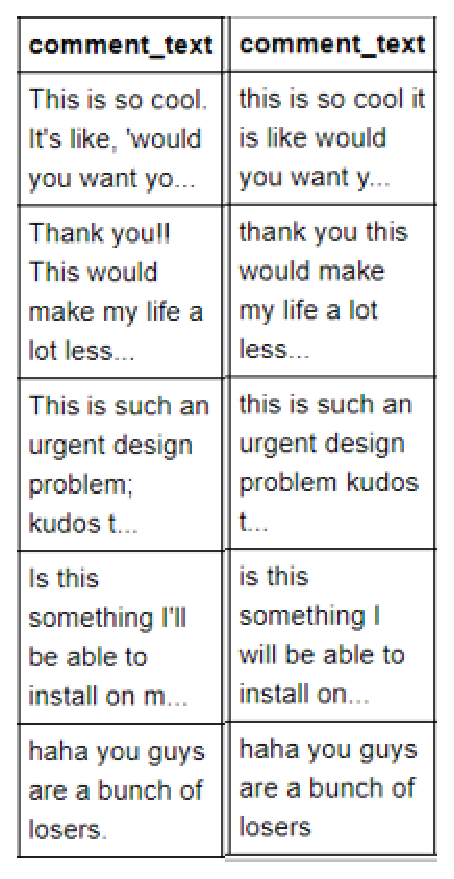
\includegraphics[scale=0.8]{picture/result.eps}
  \end{center}
}
%%%%%%%%%% -------------------------------------------------------------------- %%%%%%%%%%


% Second column - second block
%%%%%%%%%% -------------------------------------------------------------------- %%%%%%%%%%
\block[titleleft]{Conclusion}
{
 $ACC: 0.9468$

}
%%%%%%%%%% -------------------------------------------------------------------- %%%%%%%%%%



%\note[targetoffsetx=8cm, targetoffsety=-10cm,rotate=0,angle=180,radius=8cm,width=.46\textwidth,innersep=.1cm]{
%Acknowledgement
%}

%\block[titlewidthscale=0.9, bodywidthscale=0.9]
%{Acknowledgement}{
%}
%%%%%%%%%% -------------------------------------------------------------------- %%%%%%%%%%

\end{columns}


%%%%%%%%%% -------------------------------------------------------------------- %%%%%%%%%%
%[titleleft, titleoffsetx=2em, titleoffsety=1em, bodyoffsetx=2em,%
%roundedcorners=10, linewidth=0mm, titlewidthscale=0.7,%
%bodywidthscale=0.9, titlecenter]

%\colorlet{noteframecolor}{blue!20}
\colorlet{notebgcolor}{blue!20}
\colorlet{notefrcolor}{blue!20}
\note[targetoffsetx=-13cm, targetoffsety=-13cm,rotate=0,angle=180,radius=8cm,width=.96\textwidth,innersep=.4cm]
{
\begin{minipage}{0.3\linewidth}
\centering

\includegraphics[width=24cm]{logos/tulip-wordmark.eps}
\end{minipage}
\begin{minipage}{0.7\linewidth}
{ \centering
 The $11^{th}$ FLIP1
  19/07/2021, Changchun, China
}
\end{minipage}
}
%%%%%%%%%% -------------------------------------------------------------------- %%%%%%%%%%


\end{document}

%\endinput
%%
%% End of file `tikzposter-template.tex'.
